\documentclass[12pt]{article}%
\usepackage{amsmath}
\usepackage{graphicx}


\begin{document}

\newcommand\scalemath[2]{\scalebox{#1}{\mbox{\ensuremath{\displaystyle #2}}}}
\title{Machine Learning \protect\\ Assignment 2 \protect\\ CLO3 Exercise 17} 
\author{Ida Bagus Dwi Satria Kusuma \protect\\ 1301140297}
\date{\today}
\maketitle

\begin{enumerate}
	\item In this exercise we will implement SVM for linearly separable data.
	\begin{enumerate}
		\item (5 points) Load the selected data set. Visualize all data points using scatter plot. Use different color or symbol for each class. Use attribute 1 as x -axis, attribute 2 as y -axis.

		\par Berikut adalah \textit{scatter plot} dari dataset linear\_7.csv , di mana segitiga merah adalah kelas +1, dan lingkaran biru adalah kelas -1.
		\par 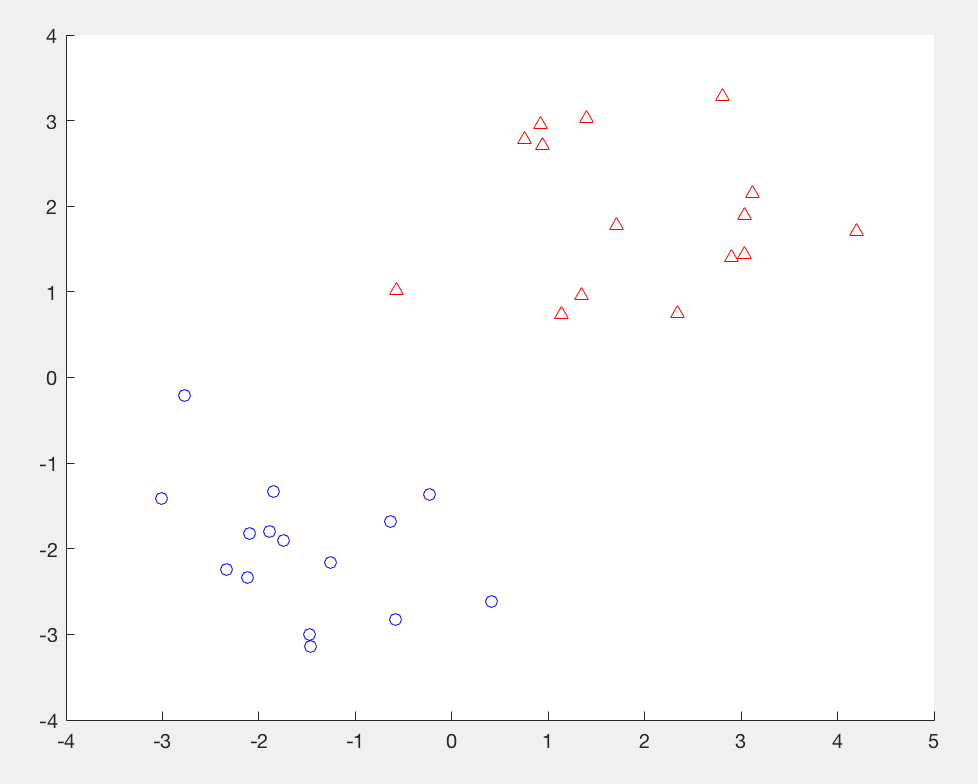
\includegraphics[width=10cm]{ass2clo3no17_1} 

		\item (20 points) Using quadratic programming library, find w and b that construct the hyperplane for classifying the selected data set.

		\par Untuk mendapatkan $\textbf{w}$ dan $b$ yang membangun \textit{hyperplane}, kita dapat menggunakan \textit{quadaratic programming}. Fungsi \textit{quadaratic programming} menyelesaikan masalah optimasi dengan bentuk : 

			\[\min _x = \frac{1}{2} \textup{x}^T \textup{Hx} + f^T\textup{x} \ \ \textup{dimana} \left\{\begin{matrix} A \cdot \textup{x} \leq b\\ Aeq \cdot \textup{x} = beq\\ lb \leq \textup{x} \leq ub \end{matrix}\right.\]

		\par Menurut [11] vektor $\textup{x} = \begin{pmatrix} \textbf{w} \\ b \end{pmatrix}$ yang dikembalikan oleh fungsi quadprog dari matlab adalah vektor berat yang kita cari untuk mendefinisikan \textit{hyperplane} yang optimal.

		\par \textit{Term} optimisasi SVM 

			\[\frac{1}{2} \begin{pmatrix} \textbf{w} & b \end{pmatrix} \begin{pmatrix} I & 0\\ 0 & 0 \end{pmatrix} \begin{pmatrix} \textbf{w}\\ b \end{pmatrix} \rightarrow \textup{min}\]

		\par dapat diformulakan dengan $\textup{H} =  \begin{pmatrix} I_n & 0\\ 0 & 0 \end{pmatrix}$ di mana $I_n$ adalah matriks identitas $n \times n$, dan $f = \begin{pmatrix} 0\\ 0\\ \vdots\\ 0 \end{pmatrix}$ adalah vektor kolom $n+1$. 0 tambahan pada ujung-kanan-bawah pada matriks identitas memastikan kita hanya meminimalkan vektor berat $\textbf{w}$ dan bukan konstan $b$.

		\par \textit{Quadratic programming} pada MATLAB memiliki parameter masukan H,f,A, dan c. nilai H dan f telah kita ketahui, namun tidak dengan nilai A dan c. Untuk mendapatkan nilai A, kita dapat membuat matriks diagonal dari data kelas dan dikalikan dengan -1, kemudian mengalikannya dengan matriks Z, yang berisi data, dengan data\_kelas $\times -1$. Sedangkan untuk c, kita membuat matriks sebanyak jumlah data, dan berisi $1 \times -1 $.

		\par Keluaran fungsi \textit{quadratic programming} adalah

			\[\textup{w} = \begin{pmatrix} 0.4111\\ 0.8994\\ 0.3236 \end{pmatrix}\]

		\par di mana $\textup{w}_1 = 0.4111$ , $\textup{w}_2 = 0.8994$, dan $b = 0.3236 $. Sehingga persamaan \textit{hyperplane}-nya adalah 

			\[hyperplane = \frac{-(0.4111\times x+0.3236)}{0.8994}\]

		\item (5 points) Now visualize the hyperplane on the scatter plot that is created on 17(a).
		\par Menggunakan persamaan \textit{hyperplane} pada nomor 17(a), garis \textit{hyperplane} dapat dilihat pada gambar

		\par 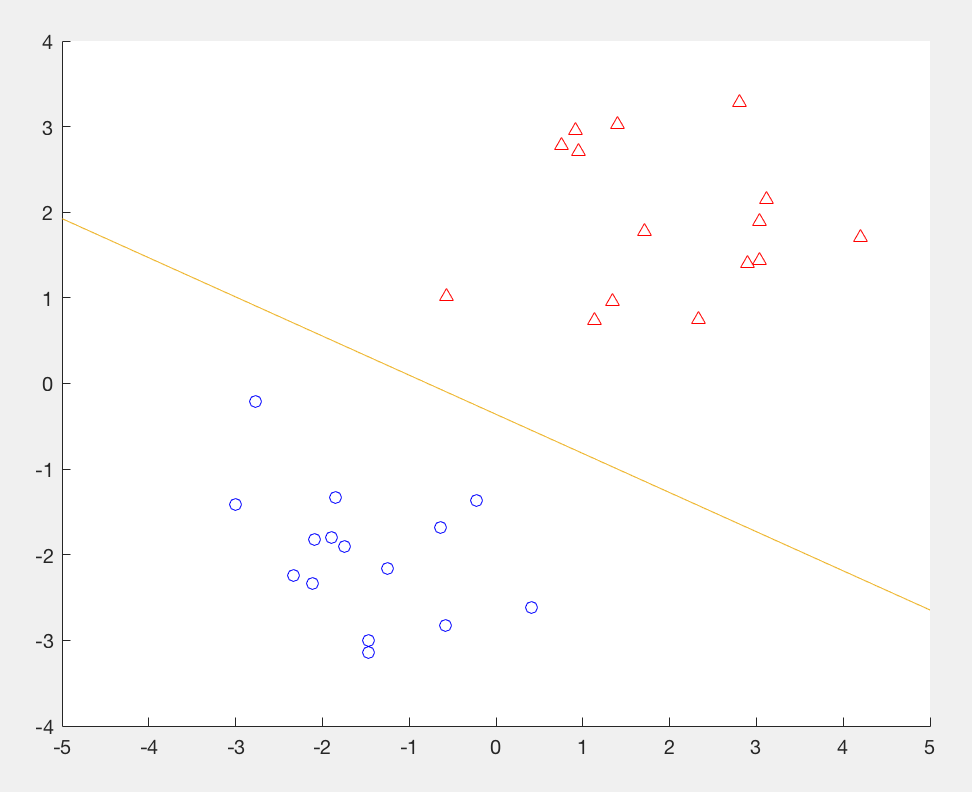
\includegraphics[width=10cm]{ass2clo3no17_3} 
	\end{enumerate}
	


\end{enumerate}

\par \textbf{Referensi}
\par [1] https://id.wikipedia.org/wiki/Regresi\_Linier
\par [2] Introduction to Data Mining - Panning Tan, M. Steinbach
\par [3] https://en.wikipedia.org/wiki/Nonlinear\_regression
\par [4] Regression book
\par [5] Regression slide
\par [6] http://www.nickgillian.com/wiki/pmwiki.php/GRT/MLP
\par [7] Machine Learning - Tom Mitchell
\par [8] https://medium.com/towards-data-science/activation-functions-and-its-types-which-is-better-a9a5310cc8f
\par [9] Slide ANN-MLP Machine Learning
\par [10] https://www.mathworks.com/help/optim/ug/quadprog.html#inputarg\_f
\par [11] http://www.robots.ox.ac.uk/~az/lectures/ml/ matlab2.pdf


\end{document}

